\chapter{Estructura digital del texto dramático}\label{chap:B2}
\epigraphhead[50]{\epigraph{Quédese vusté con Dios,\\
		ya no salgo a la comedia\\
		y ya me voy a mi casa,\\
		porque no quiere el poeta\\
		que le haga estorbo el gracioso\\
		cuando hay un paso de veras.}{Rojas Zorrilla, \textit{Peligrar en los remedios}}}
\section{Texto dramático, datos dramétricos}
En este capítulo retomamos lo visto sobre los datos y las diferentes formas de usarlos para ser aplicados a las entidades dramáticas. El objetivo ahora es definir estas como estructuras de datos, sea como elementos singulares o mediante las relaciones entre ellos. Damos por supuesto que, tras seguir lo expuesto en el capítulo anterior, disponemos ya de textos \textit{limpios} y preparados para trabajar digitalmente de modo automático.

Si bien el formato \ac{xmltei} se presta perfectamente a almacenar información y da facilidades para su manipulación, su estructura jerárquica requiere un paso intermedio para el tratamiento estadístico. Los paquetes de mayor difusión en la academia y la industria trabajan con marcos de datos\footnote{{\textit{Data frame}} en inglés.}, que no son otra cosa que una vía de abstracción para representar la sempiterna tabla. Esto es, una serie de elementos distribuidos a lo largo de filas, cuyas características se definen en columnas. De esta manera, si queremos conocer la característica $j$ del elemento $i$, nos desplazaremos verticalmente hasta la fila $i$-ésima y, en ella, miraremos el contenido de la celda correspondiente a la columna $j$-ésima.

Esto naturalmente requiere conocer en primer lugar qué características cuantificaremos para definir el formato de la tabla. También hemos de saber cómo se representarán esas características para asignarles un valor numérico o categórico, de lo que depende el formato del valor de la celda. Asimismo, necesitamos conocer qué elementos poseedores de tales características observaremos. De esta manera, nos interesa definir las entidades que constituyen la forma externa del texto dramático para poder estructurarlas después en forma tabular.

Como dijimos, estas entidades y sus relaciones estaban indicadas explícitamente en los archivos en \ac{xmltei}. Lamentablemente, no todas las fuentes se encuentran disponibles en este formato ni todas lo que lo están son fiables \parencite{valdes2014b}. Podríamos codificarlos nosotros mismos —de hecho lo haremos más adelante—, pero estaríamos en la misma tesitura porque, para hacerlo, debemos identificar primero los elementos textuales y sus relaciones.

La solución por las que nos inclinamos pasa por un sistema de tratamiento de textos semimanual. Esto es, los textos de origen se limpian primero mediante los procesos  semiautomatizados presentados en el capítulo anterior, si bien, en lugar de dejarlos tal cual, aprovechamos para que el proceso los organice según ciertas convenciones que nos resulten más convenientes. El formato nos ha de permitir identificar las entidades textuales sin ambigüedades para luego automatizar su tratamiento. Proponemos un sistema de codificación de textos dramáticos que hemos denominado Visually-Encoded Drama (\ac{ved}) para alcanzar este propósito. Hemos desarrollado este formato específicamente para el proyecto \textit{Sound and Meaning} como una aportación extra al limpiado de los textos. Esto es, surgió como una evolución de la preparación directa de los archivos, aquella consistente en eliminar información metatextual como encabezados, paginación o aparato crítico. Con unos cambios mínimos, que apenas requieren operaciones adicionales más que adaptar las ya usadas al nuevo objetivo, el texto resultante puede proporcionar información adicional sobre su estructura, así como metadatos relevantes. 

\section{De texto plano a VED}
La manipulación de las fuentes plantea varias necesidades. Por una parte, hay que disponer de un formato de representación de las ontologías propias del drama. Por otro lado, crearlo a partir del formato de partida debe implicar la mínima intervención manual. Además, todo ello debería poderse llevar a cabo sin conocimientos técnicos. De ahí el carácter visual del formato que ideamos. Este reproduce la disposición de los elementos estructurales que se hallan en la página, de manera que, al menos los concernientes al texto, pueden codificarse sin necesidad de aprendizaje (\ref{ex:vedmin}).

\begin{lstlisting}[frame=none,numbers=none,caption={Ejemplo mínimo de codificación VED.},label={ex:vedmin}]
UNO
	Es el primer verso de Uno,
	y este es uno...
OTRO
		...compartido.
	y este lo dice solo Otro.
\end{lstlisting}

Resulta evidente la similitud con el formato que encontramos en cualquier edición moderna, si bien la didascalia de personaje\index{didascalia de personaje} toma una línea\index{línea} para ella sola. Naturalmente, esta información es insuficiente, por lo que hemos de añadir otros datos de alguna manera. Nos valdremos para ello de etiquetas simples, pero siempre respetando la estructura visual del texto. Dada la flexibilidad que ofrece esta codificación, resulta sencillo construir herramientas para traducir este formato a otros, como \ac{xmltei}, por lo que también las hemos construido para llevar a cabo esta tarea. Por ahora, empezaremos por describir el formato \ac{ved} y, a continuación, explicaremos cómo llegamos hasta él.

El formato \ac{ved} está concebido con la idea de que sea intuitivo. Por lo tanto, nada mejor para explicarlo que con un ejemplo. Vemos elementos que reproducen la forma arriba descrita, así como otros menos obvios, por estar precedidos de marcas de control.  Aquí tenemos dos tipos: por un lado, etiquetas, que se asemejan a las usadas en \ac{html} o \ac{xml}, aunque, al contrario que esas codificaciones, no van por pares con una etiqueta para abrir y otra para cerrar, ya que no cumplen esa función. Al establecer una relación biunívoca entre entidad y línea, los límites de esta son los de aquella. La etiqueta, pues, solo se utiliza a efectos clasificatorios.

\begin{lstlisting}[frame=none,numbers=none,caption={Ejemplo de archivo VED.},label={ex:ved}]
<x>Comentario
<a>Autor
<t>Título
<tt>Subtítulo
<g>Género
<gg>Subgénero
<o>Obtenido de la edición tal*https://foo.bar/fuente
<f>1600-1699
<el>PERSONAS QUE HABLAN EN ELLA|Uno*Otro, otro personaje*UN TERCERO
<j>Primera Jornada
<i>Acotación
UNO #uno
	El primer verso de Uno,
	segundo, de Uno, el verso.
	Tercero es medio.
OTRO #otro
		que
UNO #uno
			sigue
	en este otro parlamento.
	<i>Acotación interna.
	Quinto verso, también fin.
UNO Y OTRO #uno \#otro
	<e>¡Fin!
<i>Vanse. Acotación externa. Entra un tercero.
TERCERO #tercero
	<i>Lee.
	<p>Esto no es un verso sino un texto en prosa.
\end{lstlisting}

Como su nombre indica, el formato \ac{ved} reproduce la estructura espacial de la pieza teatral. Se trata de un simple archivo en texto plano —por lo tanto, puede ser abierto y editado directamente en cualquier sistema sin necesidad de instalar programas adicionales—. Cada elemento textual se representa en una línea\index{línea}; estas líneas se configuran de manera interna de diferentes formas para marcar su función en el texto. Los parlamentos\index{parlamento} se distinguen de las didascalias de personaje\index{didascalias de personaje} mediante el sangrado, mientras que otras características del texto, así como el resto de acotaciones\index{acotación}, elementos textuales dramáticos inusuales y metadatos se indican mediante un reducido conjunto de etiquetas. Esto resulta en una composición legible directamente, pero semiestructurada, que se procesa automáticamente con un programa específico. Por otra parte, al remedar la disposición sobre el papel, este sistema es muy intuitivo, por lo que apenas requiere unos minutos para poder empezar a preparar textos.

Al comienzo, vemos una serie de líneas\index{línea} sin sangrar y con una etiqueta que recuerda a las que se emplean en \ac{html}. Su función es, sin embargo, un poco diferente, ya que no indica atributos sino categorías. La etiqueta \texttt{<x>} la usamos para añadir comentarios que no han de ser tenidos en cuenta en el análisis. Resulta útil cuando hay que introducir advertencias o aportar información adicional necesaria para el desarrollo del trabajo. El nombre del autor lo señalamos con la etiqueta \texttt{<a>}. Si estamos codificando la obra para procesarla e incorporarla a un corpus, sería importante convenir una forma estandarizada, de manera que varias obras del mismo autor no aparezcan con distintas variantes del nombre; el computador es incapaz de notar algo aparentemente obvio como que tanto \texttt{Calderón} como \texttt{Calderón de la Barca} y \texttt{Pedro Calderón de la Barca}, o incluso \texttt{Calderón de la Barca, Pedro}, son formas de nombrar a la misma persona. En la práctica, hemos optado por emplear versiones abreviadas del nombre en la codificación y recurrir a una tabla de conversión externa para sustituirla por el nombre completo. Aquí, confiaremos en el sentido común del lector.

Las etiquetas \texttt{<t>} y \texttt{<tt>} corresponden al título de la obra y a su subtítulo, respectivamente. La fecha la introducimos tras la etiqueta \texttt{<f>}. En el caso normal, indicamos la fecha mediante un año representado por cuatro guarismos arábigos. Si no conocemos la fecha concreta, optaremos entre usar un rango mediante dos años separados por un guion o una fecha insegura, que indicamos con un año y un signo de cierre de interrogación. Cualquier otro formato sería válido, pero, dado que no es posible contemplar todas las variantes posibles, al convertirlo a \ac{tei} produciría un formato de fecha no estandarizado. Asimismo, para dejar constancia de la procedencia editorial de la fuente, empleamos la etiqueta \texttt{<o>}. Aquí incluiremos cuantos datos estimemos convenientes y, de manera opcional, 
 una dirección de una página web asociada introducida por un asterisco. Este campo no se encuentra estandarizado, ya que no está concebido por ahora para ser estudiado, sino con fines de archivo y clasificación. Volvemos aquí a la cuestión ontológica: ¿son los datos editoriales de la edición moderna entidades susceptibles de ser estudiadas mediante la lectura distante\index{lectura distante}? Dada la falta de publicaciones que así lo consideren, lo dejaremos por ahora como un dato estrictamente metatextual no cuantificable; tal vez, habría que revisar este punto en el futuro y normalizar el formato para poder tenerlo en consideración como una variable más. 

El género y el subgénero se indican mediante \texttt{<g>} y \texttt{<gg>}. Aquí debemos considerar la misma precaución que observamos con el nombre del autor, porque el computador sería incapaz de reconocer, por ejemplo, \texttt{capa y espada} como equivalente a \texttt{de capa y espada} sin complicar el algoritmo de evaluación de los términos a comparar. Una solución eficaz consiste en asignar códigos mnemotécnicos sencillos para cada género y escribir luego de manera automática el nombre completo usando una tabla de conversión.

Tenemos además la  etiqueta \texttt{<el>} con la que introducimos el elenco. Aquí pondremos opcionalmente la cabecera que utiliza la obra para introducirlo (por ejemplo, «\textsc{Personajes que intervienen}») seguida de una barra vertical y, a continuación, los personajes. Estos van separados por asteriscos e, internamente, puede constar, además del nombre, de un epíteto opcional si lo hubiera, introducido por una coma. Conviene cuidar el detalle aquí, porque esta línea\index{línea} la emplearemos en la conversión a \ac{xmltei} no solo para los metadatos, sino para presentar las partes impresas en el cuerpo del texto. En efecto, la información necesaria para producir el bloque del cuerpo textual bajo la rama \texttt{<front>} la obtenemos a partir de la información proporcionada en estos metadatos. Gracias a ella disponemos del autor, los títulos y las \textit{dramatis personae}.

La etiqueta \texttt{<j>} señala un nuevo acto\index{acto} o jornada\index{jornada|see {acto}}. La aplicaremos incluso en obras sin macrodivisiones, pues su primera ocurrencia es la marca que señala el comienzo de la parte estructural de la obra. No existe una etiqueta específica para señalar las escenas porque no es habitual que este tipo de segmentación se señale explícitamente en las obras. A partir de aquí, comienza la representación en sí y señalamos la jerarquía estructural del texto mediante el espaciado.

Dejamos las didascalias de personaje en una línea\index{línea} sin sangrar y sin etiqueta que introduzca el texto. Podemos, además, señalar facultativamente el identificador \texttt{<xml:id>} de cada personaje para que se tenga en consideración  al convertirlo a \ac{tei}. Esto puede resultar útil cuando aparecen parlamentos\index{parlamento} colectivos, para indicar con ello quiénes toman parte. En cualquier caso, poniendo el nombre de un personaje, hemos señalado el comienzo de un nuevo parlamento. Ahora  sangraremos el texto para todo el bloque de orden jerárquico inferior supeditado a la intervención de este personaje, que incluye tanto texto como acotaciones internas\index{acotación}. Podemos encontrar versos completos o comienzos de verso\index{verso}, que no necesitan más información, ecos, que indicaremos con la etiqueta \texttt{<e>} o fragmentos en prosa, que denotamos mediante la etiqueta \texttt{<p>}. De la misma manera, si queremos señalar una acotación interna, lo indicaremos sangrando la línea antes de etiquetarla con \texttt{<i>}; para una externa, evitaríamos el sangrado. En el caso de versos compartidos, la continuación o continuaciones de un verso inconcluso se marcan con unidades de sangrado adicional para que reproduzca visualmente la edición impresa. En la práctica, dos unidades de sangrado son suficientes para el computador, pero es recomendable emplear niveles sucesivos, ya que estos ayudan a la identificación visual. Su equivalente en \ac{xmltei} lo vemos en \Cref{extendedchars:xmlved3}.

\begin{lstlisting}[frame=none,numbers=none,caption={Equivalente \ac{xmltei}.},language=xml, label={extendedchars:xmlved3}]
<sp who="#uno">
    <speaker>UNO</speaker>
    <lg>
        <l>El primer verso de Uno,</l>
        <l>segundo, de Uno, el verso.</l>
        <l part="I" >Tercero es medio.</l>
    </lg>
</sp>
<sp who="#otro">
    <speaker>OTRO</speaker>
    <lg><l part="M">que</l></lg>
</sp>
<sp who="#uno">
    <speaker>UNO</speaker>
    <lg>
        <l part="F">sigue</l>
        <l n="5">es este otro parlamento.</l>
        <stage>Acotación interna.</stage>
        <l>Quinto verso, también fin.</l>
    </lg>
</sp>
<sp who="#uno #otro">
    <speaker>UNO y OTRO</speaker>
    <lg><l>¡Fin!</l></lg>
</sp>
<stage>Vanse. Acotación externa. Entra un Tercero.</stage>
<sp who="#tercero">
    <speaker>TERCERO</speaker>
    <stage>Lee.</stage>
    <p>Esto no es un verso sino un texto en prosa</p>
</sp>
\end{lstlisting}

De esta manera, ya tendríamos nuestro texto como datos semiestructurados, lo que nos permitiría tratarlo con el computador para todo tipo de estudios cuantitativos sobre las entidades definidas. Asimismo, el formato facilitaría otras aproximaciones. Pensemos, por ejemplo, en una prueba estilométrica clásica, en la que la entidad medida es la frecuencia de las palabras. En este caso, no hemos definido esa entidad para su medición, aunque hacerlo llevaría muy pocos pasos y, además, sencillos. Considerando que los programas de estilometría toman el texto en sí como entrada, deberíamos eliminar tanto los elementos paratextuales (título de la jornada) como aquellos otros no dramatizados (acotaciones\index{acotación}...). Bastaría para esto aplicar una serie de expresiones regulares\index{expresión regular} para eliminar secuencialmente los elementos deseados. Empezaríamos, por ejemplo, por todas las líneas\index{línea} sin sangrar\index{sangrado}, luego las que empiezan con una etiqueta de acotación y, finalmente, a discreción de quien lleve a cabo la prueba, tal vez las líneas introducidas por etiquetas de prosa o eco.

\begin{lstlisting}[frame=none,numbers=none,caption={Preparación de archivo VED para análisis estilométrico.},language=bash, label={extendedchars:sed}]
	4> sed '/^\S/d' pieza.ved | sed '/<i>.*/d | sed 's/<.*>//'	 
\end{lstlisting}

Podríamos llevar una cuenta de personajes en escena según un procedimiento análogo al de determinar personajes colectivos. La aproximación más simple es incluirlos en una lista a medida que intervienen. La distribución de esta cambiaría con cada intervención, de manera que el último personaje pasaría a ocupar siempre la posición final. De esta forma, tras una acotación \textit{vase}, se sabría exactamente a quién alude. Más complicado sería \textit{Vanse}, porque atañe al menos a dos personajes, pero desconocemos a cuántos en concreto. Aproximaríamos aquí, dejando el resto a la revisión manual. Si se especifican nombres en la acotación, esta afectaría a los aludidos sin importar la posición que ocupen.  Lo vemos en \Cref{list:vanse}, donde evaluamos una lista $fuera$ indica los personajes en escena por orden de salida y la acotación. 

\begin{algorithm}[!ht]
	\caption{Personajes que se van.}\label{list:vanse}
	\Fmetodo{\EnEscena{fuera, acotación}}{
		\If{`Va[n]se' $\in$ acotación}{
			\If{$\exists personaje_i \in acotaci\acute{o}n, \forall personaje \in fuera$}{
				\fuera \gets $fuera - personaje_i$
			}
		}
		\ElseIf{`Vase' $\in$ acotación}{
			\fuera \gets $fuera_{1..n-1}$
		}
		\ElseIf{`Vanse' $\in$ acotación}{
			\fuera \gets $fuera_{1..n-2}$
		}
		\Return{fuera}	
	}
\end{algorithm}

En nuestro caso, hemos usado el procedimiento para determinar los personajes colectivos (\Cref{list2:txt2tei}), de manera que si aparece, por ejemplo, \textsc{Las dos}, serán los dos últimos personajes femeninos que han precedido la última intervención, o, si es todos, —de modo algo impreciso—, la lista entera salvo el personaje que acaba de hablar. Sin embargo, bastaría con utilizar ese valor para otros propósitos, como los descritos en \Cref{chap:ejdram} si así se desea. 

\section{Excurso \Roman{excurso}: De VED a XML-TEI}\stepcounter{excurso}
Como hemos visto, el formato \ac{ved} define una ontología que constituye un subconjunto de \ac{xmltei} y permite representar las principales entidades textuales definidas por este último para el drama. Esto facilita emplear los archivos \ac{ved} para codificar una obra y convertir la edición automáticamente a \ac{xmltei} de manera rápida, incluso sin estar familiarizado con ninguno de ambos formatos. Para llevar a cabo este proceso de transformar datos semiestructurados de forma visual en otro jerárquico no estrictamente secuencial, emplearemos el programa \texttt{text2tei} \parencite{sanz2022sc}, cuyo código fuente se encuentra en \Cref{list2:txt2tei} en su última versión a la fecha de entrega de este trabajo. Su mecanismo, a grandes rasgos, consiste en ir recorriendo las líneas\index{línea} del archivo \ac{ved} e ir asignando los valores en el lugar correspondiente de la estructura \ac{xmltei}.

Para realizar esto, definimos primero las estructuras de datos que emplearemos. Como datos de entrada, tomamos un archivo que guardamos en una variable, que separamos como una lista de sus líneas\index{línea}. Seguidamente, creamos otra variable, en la que establecemos el esqueleto de la estructura \ac{xmltei} donde colocaremos la información, con la cabecera de metadatos, los preliminares y el cuerpo del texto.

\begin{algorithm}[!ht] %or another one check
	\caption{Conversión de VED a XML-TEI.}\label{list:txt2tei}
	\vedtext \gets\ $texto.ved$\;
	\lineas \gets\ $l\acute{\imath}neas + \{l\acute{\imath}nea\} \forall l\acute{\imath}nea \in vedtext$\;
	\variables \gets\ $\{(a,\emptyset), (t, \emptyset), (tt, \emptyset), (g, \emptyset), (o, \emptyset), (f, \emptyset), (el, \emptyset)\}$\;
	\arbol \gets \CreaXML{}\;
	\arbol.\Fanade{$\{cabecera, preliminares, cuerpo\}$} \;
	\variable$_{\alpha}$ \gets\ $l\acute{\imath}nea - \alpha, \forall l\acute{\imath}nea \in vedtex \wedge l\acute{\imath}nea\: \text{\empiezacon}\: \alpha$ \;
	\variables$_{\langle f\rangle}$ \gets\ \Fdate{$variable_{\langle f\rangle}$} \;
	\variables$_{\langle a\rangle}$ \gets\ \Fautor{$metadatos_{\langle a\rangle}, tabla\_autores.xml$} \;
	\variables$_{\langle el\rangle}$ \gets\ \Fdramatis{$metadatos_{\langle el\rangle}$} \;
	\arbol.\cabecera \gets\ \Farbol{$metadatos$}\;
	\arbol.\preliminares \gets\ \Farbol{$metadatos$} \;
	\For{$l\acute{\imath}nea \in l\acute{\imath}neas$}{
		\If{$l\acute{\imath}nea\: \text{\empiezacon}\: \langle j\rangle$}{
			\arbol.\cuerpo.\Facto{}\;
		}
		\ElseIf{$\langle i\rangle \in l\acute{\imath}nea$}{
			\eIf{$l\acute{\imath}nea\:\text{\empiezacon}\: espacio$}{
				\arbol.\cuerpo.\acto.\Facotacion{$l\acute{\imath}nea - \langle i\rangle$}\;
			}
			{
				\arbol.\cuerpo.\acto.\parlamento.\Facotacion{$l\acute{\imath}nea - \langle i\rangle$} \;
			}
		}
		\ElseIf{$l\acute{\imath}nea\: \text{\empiezacon}\: letras$}{
			\arbol.\cuerpo.\Fparlamento{$l\acute{\imath}nea$} \;
		}
		\ElseIf{$l\acute{\imath}nea\: \text{\empiezacon}\: espacio$}{
			\arbol.\cuerpo.\acto.\parlamento.\Flinea{$l\acute{\imath}nea$}\;
		}
	}
\end{algorithm}

El siguiente paso será guardar los elementos de la cabecera en las variables recién definidas para manipularlas de la forma más conveniente. Así, buscamos su valor en las líneas con la etiqueta que corresponda. Como dijimos, la fecha presenta variaciones, por lo que la volvemos a evaluar para asignarle el formato preciso según se define en las directrices de \ac{tei}. Hacemos lo mismo respecto al autor y completamos el nombre consultando un archivo externo, donde tenemos la correspondiente denominación única completa de acuerdo con las convenciones de notación onomástica \ac{tei} (\Cref{list:authorsxml}). Con todos los datos de la cabecera en un formato adecuado, llenamos las ramas correspondientes en el árbol. Como ya disponemos de los componentes necesarios para completar los preliminares, lo hacemos. Con esto, tenemos listos los elementos estructurales fijos y comenzamos a tratar los variables.

Para disponer de los elementos del cuerpo del texto, iteramos por todas las líneas, ignorando, claro está, aquellas que sean comentarios. Este bucle se diferencia del anterior en que ha de introducir un número indeterminado de elementos que, a su vez, pueden contener una cantidad variable de entidades subordinadas. De esta manera, cada vez que aparezca una etiqueta señalando un nuevo acto\index{acto}, producimos un nuevo bloque en el cuerpo del texto, dentro del cual iremos construyendo las estructuras que contiene.

\begin{lstlisting}[frame=none,numbers=none,caption={Formato de autores.},language=xml, label={list:authorsxml}]
	<author cert="high">
	<persName>
	<forename>Pedro</forename>
	<surname sort="1">Calderón</surname>
	<nameLink>de la</nameLink>
	<surname>Barca</surname>
	</persName>
	<idno type="wikidata">Q170800</idno>
	<idno type="pnd">118518399</idno>
	</author>
\end{lstlisting}

 Así pues, si aparece una indicación de acotación\index{acotación}, la introduciremos como elemento hijo del acto\index{acto} con el que estamos trabajando si la etiqueta es el primer elemento de la línea o como elemento hijo de un parlamento\index{parlamento} si va precedida de algún espacio. Si la línea no empieza por espacio ni por etiqueta\footnote{Aunque no necesariamente por un carácter alfabético, ya que puede suceder que, habiendo varios personajes del mismo tipo (por ejemplo, \textsc{Pastor 1.º}, \textsc{Pastor 2.º} y \textsc{Pastor 3.º}), la didascalia de personaje se abrevie mediante el ordinal (1.º), el numeral (1) o que el editor marque un personaje implícito con corchetes ([\textsc{Pastor] 3.º}).}, será una didascalia de personaje indicando el locutor\index{locutor}; por lo tanto, creamos un nuevo parlamento en el acto dentro del que nos encontremos. Si la línea empieza con espacio, se trata de texto —de haber llevado la etiqueta de acotación, nos habría obligado a entrar en la segunda bifurcación condicional y no habríamos entrado en esta—. Para agregar la nueva línea, evaluaríamos en primer lugar si lleva etiquetas de eco o prosa, que nos obligaría a considerar de manera distinta  la cuenta de versos\index{verso}. De ir sin etiquetar, se comprobaría el sangrado para, de la misma manera, mantener invariable la numeración versal si estamos ante la continuación de un verso compartido y, además, introducir el atributo descriptivo de la parte del verso que representa tanto la línea del elemento actual como la línea precedente.

\section{Estructurando los datos}
Al tener definidas estas entidades, produciremos archivos mediante la traducción entre diferentes formatos, a condición de que compartan una misma ontología. Así, crearemos archivos \ac{ved} tomando como fuente los diferentes formatos iniciales para, a partir de ahí, por ejemplo, codificar la obra según los principios de \ac{xmltei}. De este modo, nos encontramos en condiciones de producir material que puede ser ya empleado para diversos propósitos finalistas, como representar redes de personajes, analizar la dominancia escénica y, en general, cualquiera de los análisis a mano que ilustra \Cref{chap:ejdram}. Dicho de otra manera, estos resultados resultan ya productivos por sí mismos; buena muestra de ello son las comedias de Calderón aportadas a CalDracor \parencite{caldracor2022}, todas ellas preparadas de los originales como archivos \ac{ved}, traducidos posteriormente de manera automática a \ac{xmltei} según lo descrito en este capítulo.

A pesar del valor intrínseco que pudiera tener ese resultado, es apenas un paso intermedio en este estudio. Nuestra intención es ir más allá. Téngase en cuenta que los textos en \ac{xmltei} no dejan de ser una fuente que, aunque con una estructura definida, requiere programas capaces de clasificarla y cuantificarla y de llevar a cabo cálculos partiendo de esas cuantificaciones. Si bien esto puede hacerse hoy de manera sencilla —tanto que podría darse por supuesto, ya que muchos programas orientados a ese tipo de tareas se encuentran libremente accesibles—, no deja de ser un paso intermedio que, además, está limitado a entidades y relaciones predefinidas, aparte de que su estructura jerárquica obliga a emplear \textit{trucos} cuando dos elementos estructurales concurrentes se superponen \parencite[692]{tei2022}. Nuestra intención es simplificar más aún ese análisis para poder usar los datos sin modificar en exámenes de lectura distante; esto pasa por presentar las entidades textuales cuantificadas para que los cálculos puedan hacerse de forma directa, así como extraer otra información relevante —precisamente una de especial interés para el proyecto Sound and Meaning: el ritmo—. Se trata de organizar los datos de tal manera que puedan ser leídos sin mediación por los programas más habituales de cálculo estadístico y que, además, contengan una ontología que represente los entes y relaciones que nos interesan; para ello, necesitamos no solo identificar entidades textuales, sino ordenarlas.

¿Pero cómo se traslada el formato dramático a una tabla? El modelo de los cuadros ideado por Marcus~\parencite*{marcus1973} para representar la intervención de los personajes en las obras teatrales ofrece una buena idea de cómo definir el eje temporal. Observemos el ejemplo  \Cref{fig:drama}, que sigue los principios de ese modelo: las unidades que señalan el curso de la acción son los parlamentos\index{parlamento}. A cada uno de ellos le corresponde una fila, caracterizada mediante un valor ternario por su relación con los personajes de la obra: \textit{presente hablando}, \textit{presente en silencio} y \textit{ausente}. Si bien es una aproximación aceptable, disponemos de medios para afinarla.

\begin{figure}[!ht]
	\centering\small
	\begin{tikzpicture}[ampersand replacement=\&,
	block/.style={
		anchor=center,
		minimum size=4mm,
		minimum width=4mm,
		minimum height=4mm,
		outer sep=0pt}]
	\matrix (table) [nodes in empty cells,
	matrix of nodes,
	nodes={draw, minimum size=4mm, inner sep=0pt, outer sep=0pt, anchor=center},
	row 1/.style={nodes={draw=none, anchor=west,  minimum size=4mm, rotate=90}},
	column 1/.style={nodes={draw=none, minimum size=4mm}},
	column sep=-\pgflinewidth,
	nodes=block,
	row sep=-\pgflinewidth
	]
	{
		\&\textsc{Ros.}  \&  \textsc{Clar.}  \&		\textsc{Segis.} \& \textsc{Clot.}  \&  \textsc{Sol.} \& \textsc{Ast.} \& \textsc{Estr.} \& \textsc{Damas} \& \textsc{Bas.}\& \textsc{Acom.}\\
		\&|[fill=black!100]| \& |[fill=black!27]| \&|[fill=black!0]| \& 	|[fill=black!0]| \&  |[fill=black!0 ]| \& |[fill=black!0]| \& |[fill=black!0]| \& |[fill=black!0]| \& |[fill=black!0]|\& |[fill=black!0]|\\
		\&|[fill=black!27]| \& |[fill=black!100]| \&|[fill=black!0]| \& 	|[fill=black!0]| \&  |[fill=black!0]|\& |[fill=black!0]| \& |[fill=black!0]| \& |[fill=black!0]| \& |[fill=black!0]|\& |[fill=black!0]|\\
		\&|[fill=black!100]| \& |[fill=black!27]| \&|[fill=black!0]| \& 	|[fill=black!0]| \& |[fill=black!0 ]|\& |[fill=black!0]| \& |[fill=black!0]| \& |[fill=black!0]| \& |[fill=black!0]|\& |[fill=black!0]|\\
		\&|[fill=black!27]| \& |[fill=black!100]| \&|[fill=black!0]| \& 	|[fill=black!0]| \& |[fill=black!0]|\& |[fill=black!0]| \& |[fill=black!0]| \& |[fill=black!0]| \& |[fill=black!0]|\& |[fill=black!0]|\\
		\&|[fill=black!100]| \& |[fill=black!27]| \& |[fill=black!0]| \& 	|[fill=black!0]| \&|[fill=black!0 ]|\& |[fill=black!0]| \& |[fill=black!0]| \& |[fill=black!0]| \& |[fill=black!0]|\& |[fill=black!0]|\\
		\&|[fill=black!27]| \& |[fill=black!100]| \&|[fill=black!0]| \& 	|[fill=black!0]| \& |[fill=black!0]|\& |[fill=black!0]| \& |[fill=black!0]| \& |[fill=black!0]| \& |[fill=black!0]|\& |[fill=black!0]|\\
		\&|[fill=black!100]| \& |[fill=black!27]| \&|[fill=black!0]| \& 	|[fill=black!0]| \&  |[fill=black!0 ]|\& |[fill=black!0]| \& |[fill=black!0]| \& |[fill=black!0]| \& |[fill=black!0]|\& |[fill=black!0]|\\
		\&|[fill=black!27]| \& |[fill=black!100]| \&|[fill=black!0]| \& 	|[fill=black!0]| \&  |[fill=black!0]|\& |[fill=black!0]| \& |[fill=black!0]| \& |[fill=black!0]| \& |[fill=black!0]|\& |[fill=black!0]|\\
		\&|[fill=black!100]| \& |[fill=black!27]| \&|[fill=black!0]| \& 	|[fill=black!0]| \& |[fill=black!0 ]|\& |[fill=black!0]| \& |[fill=black!0]| \& |[fill=black!0]| \& |[fill=black!0]|\& |[fill=black!0]|\\
		\&|[fill=black!27]| \& |[fill=black!100]| \&|[fill=black!0]| \& 	|[fill=black!0]| \& |[fill=black!0]|\& |[fill=black!0]| \& |[fill=black!0]| \& |[fill=black!0]| \& |[fill=black!0]|\& |[fill=black!0]|\\
		\&|[fill=black!100]| \& |[fill=black!27]| \& |[fill=black!0]| \& 	|[fill=black!0]| \&|[fill=black!0 ]|\& |[fill=black!0]| \& |[fill=black!0]| \& |[fill=black!0]| \& |[fill=black!0]|\& |[fill=black!0]|\\
		\&|[fill=black!27]| \& |[fill=black!100]| \&|[fill=black!0]| \& 	|[fill=black!0]| \& |[fill=black!0]|\& |[fill=black!0]| \& |[fill=black!0]| \& |[fill=black!0]| \& |[fill=black!0]|\& |[fill=black!0]|\\
		%
		\&|[fill=black!27]| \& |[fill=black!27]| \&|[fill=black!55]| \& 	|[fill=black!0]| \&  |[fill=black!0 ]|\& |[fill=black!0]| \& |[fill=black!0]| \& |[fill=black!0]| \& |[fill=black!0]|\& |[fill=black!0]|\\
		\&|[fill=black!100]| \& |[fill=black!27]| \&|[fill=black!0]| \& 	|[fill=black!0]| \&  |[fill=black!0 ]|\& |[fill=black!0]| \& |[fill=black!0]| \& |[fill=black!0]| \& |[fill=black!0]|\& |[fill=black!0]|\\
		\&|[fill=black!27]| \& |[fill=black!100]| \&|[fill=black!0]| \& 	|[fill=black!0]| \&  |[fill=black!0 ]|\& |[fill=black!0]| \& |[fill=black!0]| \& |[fill=black!0]| \& |[fill=black!0]|\& |[fill=black!0]|\\
		\&|[fill=black!100]| \& |[fill=black!27]| \&|[fill=black!0]| \& 	|[fill=black!0]| \&  |[fill=black!0 ]|\& |[fill=black!0]| \& |[fill=black!0]| \& |[fill=black!0]| \& |[fill=black!0]|\& |[fill=black!0]|\\
		\&	|[fill=black!27]| \& |[fill=black!100]| \&|[fill=black!0]| \& 	|[fill=black!0]| \&  |[fill=black!0 ]|\& |[fill=black!0]| \& |[fill=black!0]| \& |[fill=black!0]| \& |[fill=black!0]|\& |[fill=black!0]|\\
		\&|[fill=black!100]| \& |[fill=black!27]| \&|[fill=black!0]| \& 	|[fill=black!0]| \&  |[fill=black!0 ]|\& |[fill=black!0]| \& |[fill=black!0]| \& |[fill=black!0]| \& |[fill=black!0]|\& |[fill=black!0]|\\
		\&|[fill=black!27]| \& |[fill=black!100]| \&|[fill=black!0]| \& 	|[fill=black!0]| \&  |[fill=black!0 ]|\& |[fill=black!0]| \& |[fill=black!0]| \& |[fill=black!0]| \& |[fill=black!0]|\& |[fill=black!0]|\\
		\&|[fill=black!100]| \& |[fill=black!27]| \&|[fill=black!0]| \& 	|[fill=black!0]| \&  |[fill=black!0 ]|\& |[fill=black!0]| \& |[fill=black!0]| \& |[fill=black!0]| \& |[fill=black!0]|\& |[fill=black!0]|\\
		\&|[fill=black!27]| \& |[fill=black!27]| \&|[fill=black!100]| \& 	|[fill=black!0]| \&  |[fill=black!0 ]|\& |[fill=black!0]| \& |[fill=black!0]| \& |[fill=black!0]| \& |[fill=black!0]|\& |[fill=black!0]|\\
		\&|[fill=black!100]| \& |[fill=black!27]| \&|[fill=black!27]| \& 	|[fill=black!0]| \&  |[fill=black!0 ]|\& |[fill=black!0]| \& |[fill=black!0]| \& |[fill=black!0]| \& |[fill=black!0]|\& |[fill=black!0]|\\
		\&|[fill=black!27]| \& |[fill=black!27]| \&|[fill=black!100]| \& 	|[fill=black!0]| \&  |[fill=black!0 ]|\& |[fill=black!0]| \& |[fill=black!0]| \& |[fill=black!0]| \& |[fill=black!0]|\& |[fill=black!0]|\\
		\&|[fill=black!27]| \& |[fill=black!100]| \&|[fill=black!27]| \& 	|[fill=black!0]| \&  |[fill=black!0 ]|\& |[fill=black!0]| \& |[fill=black!0]| \& |[fill=black!0]| \& |[fill=black!0]|\& |[fill=black!0]|\\
		\&|[fill=black!100]| \& |[fill=black!27]| \&|[fill=black!27]| \& 	|[fill=black!0]| \&  |[fill=black!0 ]|\& |[fill=black!0]| \& |[fill=black!0]| \& |[fill=black!0]| \& |[fill=black!0]|\& |[fill=black!0]|\\
		\&|[fill=black!27]| \& |[fill=black!27]| \&|[fill=black!100]| \& 	|[fill=black!0]| \&  |[fill=black!0 ]|\& |[fill=black!0]| \& |[fill=black!0]| \& |[fill=black!0]| \& |[fill=black!0]|\& |[fill=black!0]|\\
		\&|[fill=black!27]| \& |[fill=black!100]| \&|[fill=black!27]| \& 	|[fill=black!0]| \&  |[fill=black!0 ]|\& |[fill=black!0]| \& |[fill=black!0]| \& |[fill=black!0]| \& |[fill=black!0]|\& |[fill=black!0]|\\
		\&|[fill=black!100]| \& |[fill=black!27]| \&|[fill=black!27]| \& 	|[fill=black!0]| \&  |[fill=black!0 ]|\& |[fill=black!0]| \& |[fill=black!0]| \& |[fill=black!0]| \& |[fill=black!0]|\& |[fill=black!0]|\\
		\&|[fill=black!27]| \& |[fill=black!27]| \&|[fill=black!100]| \& 	|[fill=black!0]| \&  |[fill=black!0 ]|\& |[fill=black!0]| \& |[fill=black!0]| \& |[fill=black!0]| \& |[fill=black!0]|\& |[fill=black!0]|\\
		\&|[fill=black!100]| \& |[fill=black!27]| \&|[fill=black!27]| \& 	|[fill=black!0]| \&  |[fill=black!0 ]|\& |[fill=black!0]| \& |[fill=black!0]| \& |[fill=black!0]| \& |[fill=black!0]|\& |[fill=black!0]|\\
		%
		\&|[fill=black!27]| \& |[fill=black!27]| \&|[fill=black!27]| \& 	|[fill=black!55]| \& |[fill=black!0]|\& |[fill=black!0]|  \& |[fill=black!0]| \& |[fill=black!0]| \& |[fill=black!0]|\& |[fill=black!0]|\\
		\&|[fill=black!100]| \& |[fill=black!27]| \&|[fill=black!27]| \& 	|[fill=black!0]| \&  |[fill=black!0]|\& |[fill=black!0]|  \& |[fill=black!0]| \& |[fill=black!0]| \& |[fill=black!0]|\& |[fill=black!0]|\\
		\&|[fill=black!27]| \& |[fill=black!27]| \&|[fill=black!100]| \& 	|[fill=black!0]| \&  |[fill=black!0]|\& |[fill=black!0]|  \& |[fill=black!0]| \& |[fill=black!0]| \& |[fill=black!0]|\& |[fill=black!0]|\\
		\&|[fill=black!27]| \& |[fill=black!27]| \&|[fill=black!27]| \& 	|[fill=black!100]| \& |[fill=black!27]|\& |[fill=black!0]|  \& |[fill=black!0]| \& |[fill=black!0]| \& |[fill=black!0]|\& |[fill=black!0]|\\
		\&|[fill=black!27]| \& |[fill=black!27]| \&|[fill=black!27]| \& 	|[fill=black!27]| \& |[fill=black!27]|\& |[fill=black!0]|  \& |[fill=black!0]| \& |[fill=black!0]| \& |[fill=black!0]|\& |[fill=black!0]|\\
		\&|[fill=black!27]| \& |[fill=black!100]| \&|[fill=black!27]| \& 	|[fill=black!27]| \& |[fill=black!27]|\& |[fill=black!0]|  \& |[fill=black!0]| \& |[fill=black!0]| \& |[fill=black!0]|\& |[fill=black!0]|\\
		\&|[fill=black!27]| \& |[fill=black!27]| \&|[fill=black!27]| \& 	|[fill=black!100]| \&  |[fill=black!27]|\& |[fill=black!0]|  \& |[fill=black!0]| \& |[fill=black!0]| \& |[fill=black!0]|\& |[fill=black!0]|\\
		\&|[fill=black!27]| \& |[fill=black!100]| \&|[fill=black!27]| \& 	|[fill=black!27]| \& |[fill=black!27]|\& |[fill=black!0]|  \& |[fill=black!0]| \& |[fill=black!0]| \& |[fill=black!0]|\& |[fill=black!0]|\\
		\&|[fill=black!27]| \& |[fill=black!27]| \&|[fill=black!27]| \& 	|[fill=black!100]| \&  |[fill=black!27]|\& |[fill=black!0]|  \& |[fill=black!0]| \& |[fill=black!0]| \& |[fill=black!0]|\& |[fill=black!0]|\\
		\&|[fill=black!27]| \& |[fill=black!27]| \&|[fill=black!100]| \& 	|[fill=black!27]| \& |[fill=black!27]|\&|[fill=black!0]|  \& |[fill=black!0]| \& |[fill=black!0]| \& |[fill=black!0]|\& |[fill=black!0]|\\
		\&|[fill=black!27]| \& |[fill=black!27]| \&|[fill=black!27]| \& 	|[fill=black!100]| \& |[fill=black!27]|\&|[fill=black!0]|  \& |[fill=black!0]| \& |[fill=black!0]| \& |[fill=black!0]|\& |[fill=black!0]|\\
		\&|[fill=black!27]| \& |[fill=black!27]| \&|[fill=black!100]| \& 	|[fill=black!27]| \& |[fill=black!27]|\& |[fill=black!0]|  \& |[fill=black!0]| \& |[fill=black!0]| \& |[fill=black!0]|\& |[fill=black!0]|\\
		\&|[fill=black!27]| \& |[fill=black!27]| \&|[fill=black!27]| \& 	|[fill=black!100]| \&  |[fill=black!27]|\& |[fill=black!0]|  \& |[fill=black!0]| \& |[fill=black!0]| \& |[fill=black!0]|\& |[fill=black!0]|\\
	};
	\node[block, label={[rotate=90]center:Escena I}, minimum size=4mm, draw, span=(table-2-1)(table-13-1)] at (fit bounding box) {};
	\node[block, label={[rotate=90]center:Escena II}, draw, span=(table-14-1)(table-31-1)] at (fit bounding box) {};
	\node[block, label={[rotate=90]center:Escena III}, draw, span=(table-32-1)(table-44-1)] at (fit bounding box) {};
\end{tikzpicture}\hspace{5mm}
\begin{tikzpicture}[ampersand replacement=\&,
	block/.style={
		anchor=center,
		minimum size=4mm,
		minimum width=4mm,
		minimum height=4mm,
		outer sep=0pt}]
	\matrix (table) [nodes in empty cells,
	matrix of nodes,
	nodes={draw, minimum size=4mm, inner sep=0pt, outer sep=0pt, anchor=center},
	row 1/.style={nodes={draw=none, anchor=west,  minimum size=4mm, rotate=90}},
	column 1/.style={nodes={draw=none, minimum size=4mm}},
	row 22/.style={nodes={draw=none, minimum height=40mm}},
	row 23/.style={nodes={draw=none}},
	row 24/.style={nodes={draw=none}},
	row 25/.style={nodes={draw=none}},
	row 26/.style={nodes={draw=none}},
	row 27/.style={nodes={draw=none, minimum height=36mm}},
	column sep=-\pgflinewidth,
	nodes=block,
	row sep=-\pgflinewidth
	]
	{         \&\textsc{Ros.}  \&  \textsc{Clar.}  \&		\textsc{Segis.} \& \textsc{Clot.}  \&  \textsc{Sol.} \& \textsc{Ast.} \& \textsc{Estr.} \& \textsc{Damas} \& \textsc{Bas.}\& \textsc{Acom.}\\                                     
		\&|[fill=black!100]| \& |[fill=black!27]| \&|[fill=black!0]| \& 	|[fill=black!27]| \& |[fill=black!27]|\& |[fill=black!0]|  \& |[fill=black!0]| \& |[fill=black!0]| \& |[fill=black!0]|\& |[fill=black!0]|\\
		\&|[fill=black!27]| \& |[fill=black!100]| \&|[fill=black!0]| \& 	|[fill=black!27]| \& |[fill=black!27]|\& |[fill=black!0]|  \& |[fill=black!0]| \& |[fill=black!0]| \& |[fill=black!0]|\& |[fill=black!0]|\\
		\&|[fill=black!27]| \& |[fill=black!27]| \&|[fill=black!0]| \& 	|[fill=black!100]| \& |[fill=black!27]|\& |[fill=black!0]|  \& |[fill=black!0]| \& |[fill=black!0]| \& |[fill=black!0]|\& |[fill=black!0]|\\
		\&|[fill=black!27]| \& |[fill=black!27]| \&|[fill=black!0]| \& 	|[fill=black!27]| \& |[fill=black!100]|\& |[fill=black!0]|  \& |[fill=black!0]| \& |[fill=black!0]| \& |[fill=black!0]|\& |[fill=black!0]|\\
		\&|[fill=black!27]| \& |[fill=black!27]| \&|[fill=black!0]| \& 	|[fill=black!100]| \& |[fill=black!27]|\& |[fill=black!0]|  \& |[fill=black!0]| \& |[fill=black!0]| \& |[fill=black!0]|\& |[fill=black!0]|\\
		\&|[fill=black!100]| \& |[fill=black!27]| \&|[fill=black!0]| \& 	|[fill=black!27]| \& |[fill=black!27]|\& |[fill=black!0]|  \& |[fill=black!0]| \& |[fill=black!0]| \& |[fill=black!0]|\& |[fill=black!0]|\\
		\&|[fill=black!27]| \& |[fill=black!100]| \&|[fill=black!0]| \& 	|[fill=black!27]| \& |[fill=black!27]|\& |[fill=black!0]|  \& |[fill=black!0]| \& |[fill=black!0]| \& |[fill=black!0]|\& |[fill=black!0]|\\
		\&|[fill=black!100]| \& |[fill=black!27]| \&|[fill=black!0]| \& 	|[fill=black!27]| \& |[fill=black!27]|\& |[fill=black!0]|  \& |[fill=black!0]| \& |[fill=black!0]| \& |[fill=black!0]|\& |[fill=black!0]|\\
		\&|[fill=black!27]| \& |[fill=black!27]| \&|[fill=black!0]| \& 	|[fill=black!100]| \& |[fill=black!27]|\& |[fill=black!0]|  \& |[fill=black!0]| \& |[fill=black!0]| \& |[fill=black!0]|\& |[fill=black!0]|\\
		\&|[fill=black!100]| \& |[fill=black!27]| \&|[fill=black!0]| \& 	|[fill=black!27]| \& |[fill=black!27]|\& |[fill=black!0]|  \& |[fill=black!0]| \& |[fill=black!0]| \& |[fill=black!0]|\& |[fill=black!0]|\\
		\&|[fill=black!27]| \& |[fill=black!27]| \&|[fill=black!0]| \& 	|[fill=black!100]| \& |[fill=black!27]|\& |[fill=black!0]|  \& |[fill=black!0]| \& |[fill=black!0]| \& |[fill=black!0]|\& |[fill=black!0]|\\
		\&|[fill=black!100]| \& |[fill=black!27]| \&|[fill=black!0]| \& 	|[fill=black!27]| \& |[fill=black!27]|\& |[fill=black!0]|  \& |[fill=black!0]| \& |[fill=black!0]| \& |[fill=black!0]|\& |[fill=black!0]|\\
		\&|[fill=black!27]| \& |[fill=black!27]| \&|[fill=black!0]| \& 	|[fill=black!100]| \& |[fill=black!27]|\& |[fill=black!0]|  \& |[fill=black!0]| \& |[fill=black!0]| \& |[fill=black!0]|\& |[fill=black!0]|\\
		\&|[fill=black!100]| \& |[fill=black!27]| \&|[fill=black!0]| \& 	|[fill=black!27]| \& |[fill=black!27]|\& |[fill=black!0]|  \& |[fill=black!0]| \& |[fill=black!0]| \& |[fill=black!0]|\& |[fill=black!0]|\\
		\&|[fill=black!27]| \& |[fill=black!27]| \&|[fill=black!0]| \& 	|[fill=black!100]| \& |[fill=black!27]|\& |[fill=black!0]|  \& |[fill=black!0]| \& |[fill=black!0]| \& |[fill=black!0]|\& |[fill=black!0]|\\
		%
		\&|[fill=black!0]| \& |[fill=black!0]| \&|[fill=black!0]| \& 	|[fill=black!0]| \&  |[fill=black!27 ]| \& |[fill=black!100]| \& |[fill=black!27]| \& |[fill=black!27]| \& |[fill=black!0]|\& |[fill=black!0]|\\	
		\&|[fill=black!0]| \& |[fill=black!0]| \&|[fill=black!0]| \& 	|[fill=black!0]| \&  |[fill=black!27 ]| \& |[fill=black!27]| \& 
		|[fill=black!100]| \& |[fill=black!27]| \& |[fill=black!0]|\& |[fill=black!0]|\\			
		\&|[fill=black!0]| \& |[fill=black!0]| \&|[fill=black!0]| \& 	|[fill=black!0]| \&  |[fill=black!27 ]| \& |[fill=black!100]| \& 
		|[fill=black!27]| \& |[fill=black!27]| \& |[fill=black!0]|\& |[fill=black!0]|\\			
		\&|[fill=black!0]| \& |[fill=black!0]| \&|[fill=black!0]| \& 	|[fill=black!0]| \&  |[fill=black!27 ]| \& |[fill=black!27]| \& 
		|[fill=black!100]| \& |[fill=black!27]| \& |[fill=black!0]|\& |[fill=black!0]|\\			
		\&|[fill=black!0]| \& |[fill=black!0]| \&|[fill=black!0]| \& 	|[fill=black!0]| \&  |[fill=black!27 ]| \& |[fill=black!100]| \& 
		|[fill=black!27]| \& |[fill=black!27]| \& |[fill=black!0]|\& |[fill=black!0]|\\
		%
	     \&\&\&\&\&\&\&\&\&\&\\ 
	    \&\&\&|[draw, fill=black!100]|\&\&\&\&\&\&\&\\  
	    \&\&\&|[draw, fill=black!27]|\&\&\&\&\&\&\&\\ 
	    \&\&\&|[draw, fill=black!55]|\&\&\&\&\&\&\&\\  
	    \&\&\&|[draw, fill=black!0]| \&\&\&\&\&\&\&\\
	    \&\&\&\&\&\&\&\&\&\&\\  
	};
	\node[block, label={[rotate=90]center:Escena IV}, minimum size=4mm, draw, span=(table-2-1)(table-16-1)] at (fit bounding box) {};
	\node[block, label={[rotate=90]center:Escena V}, minimum size=4mm, draw, span=(table-17-1)(table-21-1)] at (fit bounding box) {};
	\node[block, anchor=west, minimum size=4mm, span=(table-23-4)(table-23-6)] at (fit bounding box) {Habla};
	\node[block, anchor=west, label={}, minimum size=4mm, span=(table-24-4)(table-24-6)] at (fit bounding box) {Presente};
	\node[block, anchor=west, minimum size=4mm, span=(table-25-4)(table-25-6)] at (fit bounding box) {Habla dentro};
	\node[block,anchor=west,  minimum size=4mm, span=(table-26-4)(table-26-6)] at (fit bounding box) {Ausente};
	\end{tikzpicture}\hspace{5mm}
\begin{tikzpicture}[ampersand replacement=\&,
	block/.style={
	anchor=center,
	minimum size=4mm,
	minimum width=4mm,
	minimum height=4mm,
	outer sep=0pt}]
	\matrix (table) [nodes in empty cells,
	matrix of nodes,
	nodes={draw, minimum size=4mm, inner sep=0pt, outer sep=0pt, anchor=center},
	row 1/.style={nodes={draw=none, anchor=west,  minimum size=4mm, rotate=90}},
	column 1/.style={nodes={draw=none, minimum size=4mm}},
	column sep=-\pgflinewidth,
	nodes=block,
	row sep=-\pgflinewidth
	]
	{
			\&\textsc{Ros.}  \&  \textsc{Clar.}  \&		\textsc{Segis.} \& \textsc{Clot.}  \&  \textsc{Sol.} \& \textsc{Ast.} \& \textsc{Estr.} \& \textsc{Damas} \& \textsc{Bas.}\& \textsc{Acom.}\\
		\&|[fill=black!0]| \& |[fill=black!0]| \&|[fill=black!0]| \& 	|[fill=black!0]| \&  |[fill=black!27 ]|\& |[fill=black!27]| \& |[fill=black!100]| \& |[fill=black!27]| \& |[fill=black!27]| \& |[fill=black!27]|\\
		\&|[fill=black!0]| \& |[fill=black!0]| \&|[fill=black!0]| \& 	|[fill=black!0]| \&  |[fill=black!27 ]|\& |[fill=black!100]| \& |[fill=black!27]| \& |[fill=black!27]| \& |[fill=black!27]| \& |[fill=black!27]|\\
		\&|[fill=black!0]| \& |[fill=black!0]| \&|[fill=black!0]| \& 	|[fill=black!0]| \&  |[fill=black!27 ]|\& |[fill=black!27]| \& |[fill=black!100]| \& |[fill=black!27]| \& |[fill=black!27]| \& |[fill=black!27]|\\
		\&|[fill=black!0]| \& |[fill=black!0]| \&|[fill=black!0]| \& 	|[fill=black!0]| \&  |[fill=black!27 ]|\& |[fill=black!100]| \& |[fill=black!27]| \& |[fill=black!27]| \& |[fill=black!27]| \& |[fill=black!27]|\\
		\&|[fill=black!0]| \& |[fill=black!0]| \&|[fill=black!0]| \& 	|[fill=black!0]| \&  |[fill=black!27 ]|\& |[fill=black!27]| \& |[fill=black!100]| \& |[fill=black!27]| \& |[fill=black!27]| \& |[fill=black!27]|\\
		\&|[fill=black!0]| \& |[fill=black!0]| \&|[fill=black!0]| \& 	|[fill=black!0]| \&  |[fill=black!27 ]|\& |[fill=black!100]| \& |[fill=black!27]| \& |[fill=black!27]| \& |[fill=black!27]| \& |[fill=black!27]|\\
		\&|[fill=black!0]| \& |[fill=black!0]| \&|[fill=black!0]| \& 	|[fill=black!0]| \&  |[fill=black!27 ]|\& |[fill=black!27]| \& |[fill=black!100]| \& |[fill=black!27]| \& |[fill=black!27]| \& |[fill=black!27]|\\
		\&|[fill=black!0]| \& |[fill=black!0]| \&|[fill=black!0]| \& 	|[fill=black!0]| \&  |[fill=black!27 ]|\& |[fill=black!100]| \& |[fill=black!27]| \& |[fill=black!27]| \& |[fill=black!27]| \& |[fill=black!27]|\\
		\&|[fill=black!0]| \& |[fill=black!0]| \&|[fill=black!0]| \& 	|[fill=black!0]| \&  |[fill=black!27 ]|\& |[fill=black!27]| \& |[fill=black!100]| \& |[fill=black!27]| \& |[fill=black!27]| \& |[fill=black!27]|\\
		\&|[fill=black!0]| \& |[fill=black!0]| \&|[fill=black!0]| \& 	|[fill=black!0]| \&  |[fill=black!27 ]|\& |[fill=black!100]| \& |[fill=black!27]| \& |[fill=black!27]| \& |[fill=black!27]| \& |[fill=black!27]|\\
		\&|[fill=black!0]| \& |[fill=black!0]| \&|[fill=black!0]| \& 	|[fill=black!0]| \&  |[fill=black!27 ]|\& |[fill=black!27]| \& |[fill=black!100]| \& |[fill=black!27]| \& |[fill=black!27]| \& |[fill=black!27]|\\
		\&|[fill=black!0]| \& |[fill=black!0]| \&|[fill=black!0]| \& 	|[fill=black!0]| \&  |[fill=black!27 ]|\& |[fill=black!100]| \& |[fill=black!27]| \& |[fill=black!27]| \& |[fill=black!27]| \& |[fill=black!27]|\\
		\&|[fill=black!0]| \& |[fill=black!0]| \&|[fill=black!0]| \& 	|[fill=black!0]| \&  |[fill=black!27 ]|\& |[fill=black!27]| \& |[fill=black!100]| \& |[fill=black!27]| \& |[fill=black!27]| \& |[fill=black!27]|\\
		\&|[fill=black!0]| \& |[fill=black!0]| \&|[fill=black!0]| \& 	|[fill=black!0]| \&  |[fill=black!27 ]|\& |[fill=black!100]| \& |[fill=black!27]| \& |[fill=black!27]| \& |[fill=black!27]| \& |[fill=black!27]|\\
		\&|[fill=black!0]| \& |[fill=black!0]| \&|[fill=black!0]| \& 	|[fill=black!0]| \&  |[fill=black!27 ]|\& |[fill=black!027]| \& |[fill=black!27]| \& |[fill=black!27]| \& |[fill=black!100]| \& |[fill=black!27]|\\
		\&|[fill=black!0]| \& |[fill=black!0]| \&|[fill=black!0]| \& 	|[fill=black!0]| \&  |[fill=black!27 ]|\& |[fill=black!100]| \& |[fill=black!27]| \& |[fill=black!27]| \& |[fill=black!27]| \& |[fill=black!27]|\\
		\&|[fill=black!0]| \& |[fill=black!0]| \&|[fill=black!0]| \& 	|[fill=black!0]| \&  |[fill=black!100]|\& |[fill=black!100]| \& |[fill=black!100]| \& |[fill=black!100]| \& |[fill=black!27]| \& |[fill=black!100]|\\
		\&|[fill=black!0]| \& |[fill=black!0]| \&|[fill=black!0]| \& 	|[fill=black!0]| \&  |[fill=black!27 ]|\& |[fill=black!027]| \& |[fill=black!27]| \& |[fill=black!27]| \& |[fill=black!100]| \& |[fill=black!27]|\\
		\&|[fill=black!0]| \& |[fill=black!0]| \&|[fill=black!0]| \& 	|[fill=black!0]| \&  |[fill=black!100 ]|\& |[fill=black!100]| \& |[fill=black!100]| \& |[fill=black!100]| \& |[fill=black!27]| \& |[fill=black!100]|\\
		% 
		\&|[fill=black!27]| \& |[fill=black!27]| \&|[fill=black!0]| \& 	|[fill=black!100]| \&  |[fill=black!0 ]|\& |[fill=black!0]| \& |[fill=black!0]| \& |[fill=black!0]| \& |[fill=black!27]| \& |[fill=black!0]|\\
		\&|[fill=black!27]| \& |[fill=black!27]| \&|[fill=black!0]| \& 	|[fill=black!27]| \&  |[fill=black!0 ]|\& |[fill=black!0]| \& |[fill=black!0]| \& |[fill=black!0]| \& |[fill=black!100]| \& |[fill=black!0]|\\
		\&|[fill=black!27]| \& |[fill=black!27]| \&|[fill=black!0]| \& 	|[fill=black!100]| \&  |[fill=black!0 ]|\& |[fill=black!0]| \& |[fill=black!0]| \& |[fill=black!0]| \& |[fill=black!27]| \& |[fill=black!0]|\\
		\&|[fill=black!27]| \& |[fill=black!27]| \&|[fill=black!0]| \& 	|[fill=black!27]| \&  |[fill=black!0 ]|\& |[fill=black!0]| \& |[fill=black!0]| \& |[fill=black!0]| \& |[fill=black!100]| \& |[fill=black!0]|\\
		\&|[fill=black!27]| \& |[fill=black!27]| \&|[fill=black!0]| \& 	|[fill=black!100]| \&  |[fill=black!0 ]|\& |[fill=black!0]| \& |[fill=black!0]| \& |[fill=black!0]| \& |[fill=black!27]| \& |[fill=black!0]|\\
		\&|[fill=black!27]| \& |[fill=black!27]| \&|[fill=black!0]| \& 	|[fill=black!27]| \&  |[fill=black!0 ]|\& |[fill=black!0]| \& |[fill=black!0]| \& |[fill=black!0]| \& |[fill=black!100]| \& |[fill=black!0]|\\
		\&|[fill=black!27]| \& |[fill=black!27]| \&|[fill=black!0]| \& 	|[fill=black!100]| \&  |[fill=black!0 ]|\& |[fill=black!0]| \& |[fill=black!0]| \& |[fill=black!0]| \& |[fill=black!27]| \& |[fill=black!0]|\\
		\&|[fill=black!27]| \& |[fill=black!27]| \&|[fill=black!0]| \& 	|[fill=black!27]| \&  |[fill=black!0 ]|\& |[fill=black!0]| \& |[fill=black!0]| \& |[fill=black!0]| \& |[fill=black!100]| \& |[fill=black!0]|\\
		\&|[fill=black!27]| \& |[fill=black!27]| \&|[fill=black!0]| \& 	|[fill=black!100]| \&  |[fill=black!0 ]|\& |[fill=black!0]| \& |[fill=black!0]| \& |[fill=black!0]| \& |[fill=black!27]| \& |[fill=black!0]|\\
		%                              
		\&|[fill=black!27]| \& |[fill=black!27]| \&|[fill=black!0]| \& 	|[fill=black!100]| \&  |[fill=black!0 ]|\& |[fill=black!0]| \& |[fill=black!0]| \& |[fill=black!0]| \& |[fill=black!0]| \& |[fill=black!0]|\\
		\&|[fill=black!100]| \& |[fill=black!27]| \&|[fill=black!0]| \& 	|[fill=black!27]| \&  |[fill=black!0 ]|\& |[fill=black!0]| \& |[fill=black!0]| \& |[fill=black!0]| \& |[fill=black!0]| \& |[fill=black!0]|\\
		\&|[fill=black!27]| \& |[fill=black!100]| \&|[fill=black!0]| \& 	|[fill=black!27]| \&  |[fill=black!0 ]|\& |[fill=black!0]| \& |[fill=black!0]| \& |[fill=black!0]| \& |[fill=black!0]| \& |[fill=black!0]|\\
		\&|[fill=black!100]| \& |[fill=black!27]| \&|[fill=black!0]| \& 	|[fill=black!27]| \&  |[fill=black!0 ]|\& |[fill=black!0]| \& |[fill=black!0]| \& |[fill=black!0]| \& |[fill=black!0]| \& |[fill=black!0]|\\
		\&	|[fill=black!27]| \& |[fill=black!27]| \&|[fill=black!0]| \& 	|[fill=black!100]| \&  |[fill=black!0 ]|\& |[fill=black!0]| \& |[fill=black!0]| \& |[fill=black!0]| \& |[fill=black!0]| \& |[fill=black!0]|\\
		\&|[fill=black!100]| \& |[fill=black!27]| \&|[fill=black!0]| \& 	|[fill=black!27]| \&  |[fill=black!0 ]|\& |[fill=black!0]| \& |[fill=black!0]| \& |[fill=black!0]| \& |[fill=black!0]| \& |[fill=black!0]|\\
		\&|[fill=black!27]| \& |[fill=black!27]| \&|[fill=black!0]| \& 	|[fill=black!100]| \&  |[fill=black!0 ]|\& |[fill=black!0]| \& |[fill=black!0]| \& |[fill=black!0]| \& |[fill=black!0]| \& |[fill=black!0]|\\
		\&|[fill=black!100]| \& |[fill=black!27]| \&|[fill=black!0]| \& 	|[fill=black!27]| \&  |[fill=black!0 ]|\& |[fill=black!0]| \& |[fill=black!0]| \& |[fill=black!0]| \& |[fill=black!0]| \& |[fill=black!0]|\\
		\&|[fill=black!27]| \& |[fill=black!27]| \&|[fill=black!0]| \& 	|[fill=black!100]| \&  |[fill=black!0 ]|\& |[fill=black!0]| \& |[fill=black!0]| \& |[fill=black!0]| \& |[fill=black!0]| \& |[fill=black!0]|\\
		\&|[fill=black!100]| \& |[fill=black!27]| \&|[fill=black!0]| \& 	|[fill=black!27]| \&  |[fill=black!0 ]|\& |[fill=black!0]| \& |[fill=black!0]| \& |[fill=black!0]| \& |[fill=black!0]| \& |[fill=black!0]|\\
		\&|[fill=black!27]| \& |[fill=black!27]| \&|[fill=black!0]| \& 	|[fill=black!100]| \&  |[fill=black!0 ]|\& |[fill=black!0]| \& |[fill=black!0]| \& |[fill=black!0]| \& |[fill=black!0]| \& |[fill=black!0]|\\
		\&|[fill=black!100]| \& |[fill=black!27]| \&|[fill=black!0]| \& 	|[fill=black!27]| \&  |[fill=black!0 ]|\& |[fill=black!0]| \& |[fill=black!0]| \& |[fill=black!0]| \& |[fill=black!0]| \& |[fill=black!0]|\\
		\&|[fill=black!27]| \& |[fill=black!27]| \&|[fill=black!0]| \& 	|[fill=black!100]| \&  |[fill=black!0 ]|\& |[fill=black!0]| \& |[fill=black!0]| \& |[fill=black!0]| \& |[fill=black!0]| \& |[fill=black!0]|\\
		\&|[fill=black!100]| \& |[fill=black!27]| \&|[fill=black!0]| \& 	|[fill=black!27]| \&  |[fill=black!0 ]|\& |[fill=black!0]| \& |[fill=black!0]| \& |[fill=black!0]| \& |[fill=black!0]| \& |[fill=black!0]|\\
		\&|[fill=black!27]| \& |[fill=black!27]| \&|[fill=black!0]| \& 	|[fill=black!100]| \&  |[fill=black!0 ]|\& |[fill=black!0]| \& |[fill=black!0]| \& |[fill=black!0]| \& |[fill=black!0]| \& |[fill=black!0]|\\
		\&|[fill=black!100]| \& |[fill=black!27]| \&|[fill=black!0]| \& 	|[fill=black!27]| \&  |[fill=black!0 ]|\& |[fill=black!0]| \& |[fill=black!0]| \& |[fill=black!0]| \& |[fill=black!0]| \& |[fill=black!0]|\\
		\&|[fill=black!27]| \& |[fill=black!27]| \&|[fill=black!0]| \& 	|[fill=black!100]| \&  |[fill=black!0 ]|\& |[fill=black!0]| \& |[fill=black!0]| \& |[fill=black!0]| \& |[fill=black!0]| \& |[fill=black!0]|\\
		\&|[fill=black!100]| \& |[fill=black!27]| \&|[fill=black!0]| \& 	|[fill=black!27]| \&  |[fill=black!0 ]|\& |[fill=black!0]| \& |[fill=black!0]| \& |[fill=black!0]| \& |[fill=black!0]| \& |[fill=black!0]|\\
		\&	|[fill=black!0]| \& |[fill=black!0]| \&|[fill=black!0]| \& 	|[fill=black!100]| \&  |[fill=black!0 ]|\& |[fill=black!0]| \& |[fill=black!0]| \& |[fill=black!0]| \& |[fill=black!0]| \& |[fill=black!0]|\\                 	
	};
\node[block, label={[rotate=90]center:Escena VI}, draw, span=(table-2-1)(table-20-1)] at (fit bounding box) {};
\node[block, label={[rotate=90]center:Escena VII}, draw, span=(table-21-1)(table-29-1)] at (fit bounding box) {};
\node[block,  label={[rotate=90]center:Escena VIII}, draw, span=(table-30-1)(table-48-1)] at (fit bounding box) {};
\end{tikzpicture}\relax

	\caption{Estructura de la configuración dramática.}
	\label{fig:drama}
\end{figure}

En efecto, en la obra teatral áurea, el texto se dispone en líneas\index{línea}, por lo que el transcurso del tiempo se divide en unidades discretas. Está claro que no es una medida exacta, en tanto que el teatro es polimétrico y, por ejemplo, un verso\index{verso} hexasílabo será métricamente más breve que un endecasílabo y las líneas acusaran normalmente la desproporción de igual manera. Asimismo, la acción dramática determina la cadencia de la declamación, por lo que dos líneas idénticas en el papel pueden realizarse más o menos aprisa sobre las tablas. Por lo tanto, trabajamos con una idealización en la que suponemos la línea como una medida abstracta del paso del tiempo escénico. Definimos, en cualquier caso, una ontología en la que existe esta clase línea ($L$), con tantos individuos $l_i$ ordenados sucesivamente como líneas tenga la obra, tal que $l_i \prec l_{i+1}$. De esta manera, encontraríamos en el índice una relación fundamental entre las entidades que hemos definido, pues indicaría la posición única en el tiempo de cada línea. 

¿Cómo caracterizar la línea? Podríamos hacerlo a la manera de Marcus, pero nos topamos con el inconveniente de que cada pieza requeriría un formato de tabla propio, lo que complicaría trabajar con un corpus de obras teatrales. Debemos, por lo tanto, unificar las columnas para que sean las mismas para todas las obras. Por otra parte, como ya indicamos, no disponemos de información detallada sobre la presencia escénica, por lo que resultaría harto complicado determinarla automáticamente, y tremendamente costoso en recursos llevarlo a cabo de manera manual. La alternativa que proponemos es considerar una sola columna categórica, cuyos valores son los nombres de los personajes de las obras, y que acepte la composición de categorías. Esto es, adoptaría valores como \textsc{Rosaura} o \textsc{Clarín}, pero también tomaría el valor $\textsc{Rosaura} \oplus \textsc{Clarín}$, si la didascalia de personaje\index{didascalia de personaje} indica que hablan los dos.

Por otra parte, el propio texto de la línea podría ser un valioso atributo que nos ayudaría a establecer relaciones léxicas y semánticas. Asimismo, al tener personajes, deberíamos añadir columnas con información adicional. Si bien hay nombres de personaje que son prototípicos —raro es que un \textit{Chichón} no sea un gracioso—, hay otros más comunes que pueden aparecer representando tipologías distintas en diferentes obras. Por otro lado, es posible que el sexo sea ambiguo. Por lo tanto, no asumiremos una identificación preestablecida, sino que conviene indicarla en función de la obra. Para ello, necesitaremos columnas al efecto. Si bien el sexo de los personajes resulta sencillo de predecir de forma automática en muchos casos, cuando se indica mediante un nombre de uso habitual, va antecedido por un título de cortesía o un artículo —al menos en singular, ya que resulta complicado no pocas veces, incluso leyendo, distinguir si el plural es masculino o neutro—, la tipología del personaje lo es menos si no se indica en la presentación del elenco.

Debemos, además, tener en cuenta que no todos los elementos textuales son líneas propiamente dichas y hay algunos fuera de la diégesis. En concreto, las acotaciones\index{acotación} no solo no corresponden a personajes, sino que tampoco ocupan un lapso de tiempo, por lo que van paralelos a la acción. Necesitamos incluirlos de tal manera que esto se tenga en cuenta. A despecho de forzar la terminología —en pro de la sencillez, añadiremos en nuestro descargo—, incluiremos estos elementos en la ahora difusa clase de las \textit{líneas}. Para ello, podríamos definir un nuevo atributo con una numeración alternativa al índice. Así podría llevarse la cuenta si se van marcando las acotaciones con números negativos decrementales para ordenarlas entre sí o ubicarlas de acuerdo con los versos\index{verso}. No obstante, esto resulta redundante porque disponemos de suficiente información con los atributos que representan el índice y el personaje. Si a este último, por ejemplo, lo denominamos \textsc{Acotación}, sabríamos tanto su ubicación exacta como que la línea\index{línea} es extradiegética. 

De la misma manera, dadas las características del drama áureo, podríamos incluir una segunda numeración adicional que nos indique el número de verso\index{verso}. Así, en uno compartido, el valor de los atributos para el índice y línea\index{línea} avanza con cada individuo, mientras que el que indica el verso permanece invariable hasta superar la última parte del verso actual. En el caso excepcional de que sea una línea extradiegética o un parlamento\index{parlamento} en prosa, el atributo estaría vacío; formalmente, $v_{i} \preceq v_{i+1} \vee v_{i} = \emptyset$.

Al contrario que en \ac{xmltei}, donde los metadatos se indican una sola vez, el formato tabular demandaría que se repitieran en cada fila de la obra, en tanto que estos datos afectan a todos los versos\index{verso}. El autor y el título de la obra, información de la edición, fechas, categorización genérica o el subtítulo, son elementos que se contarían entre los invariables dentro de la obra. Debemos tener cuidado aquí de que la distinción sea efectiva. Por consiguiente, no está de más contar con una columna de subgénero y subtítulo, de manera que si el título es \textit{La vida es sueño}, sepamos si nos encontramos ante la tragedia o el auto sacramental homónimo y, en este último caso, poder identificar la versión.

\section{Implementación del proceso}

Veamos, pues, cómo plasmamos esto en una representación formal. Recordemos que partimos de un texto en formato \ac{ved}. Nuestro objetivo es obtener a partir de él una tabla de \textit{líneas}\index{línea}\footnote{Usaremos letra redonda para la línea dramática en propiedad y cursiva para la entidad abstracta que hemos definido, que comprende acotaciones además de estas.}, cuyos atributos nos permitan caracterizarlas de tal manera que sea posible realizar con ellas análisis cuantitativos directamente. Empezaremos definiendo los atributos de la línea y asignándoles un valor por defecto. Antes de empezar a recorrerlas, no tenemos definido un acto\index{acto}, parlamento\index{parlamento} o verso\index{verso}, sino que cobran entidad al leer la primera \textit{línea}. Por lo tanto, estarán a cero hasta entonces. Definimos asimismo variables auxiliares para llevar la cuenta de los parlamentos y las acotaciones\index{acotación} por separado. Los atributos de la clase, al no tener ninguna instancia de esta aún, estarán también a cero, salvo el locutor\index{locutor}, que pondremos como \textit{acotación}. Esto es, como habíamos decidido, la acotación es una instancia especial de la clase \textit{línea}, que se diferencia de las partes habladas por su locutor y por tener número de línea negativo.

\begin{algorithm}[!ht]
	\caption{Cabecera para la tabulación.}\label{list:normal1}
	\acto, \parlamento, \verso, \nparlamento, \nacotacion  \gets 0 \;
	\p \gets $'\emptyset'$ \;
	\autor, \titulo, \genero, \sexo, \s, \edicion, \fecha \gets $\emptyset$ \;
	\personaje \gets \textsc{Acotación} \;
	\tabla \gets \Tabla{\{Autor, Título, Subt., Género, Subg., Edición, Fecha, Jornada, Parlamento, Verso, Locutor, Tipo, Sexo, Texto\}} \;
	\nombres \gets $\{\emptyset\}$ \;
\end{algorithm}

Después de esto, pasaremos a predecir el sexo de los personajes. El método comete errores y necesita una revisión manual en cualquier caso. Sin embargo, dada la relativa predictibilidad de la onomástica hispana, el porcentaje de fallos se reduce hasta el punto de aliviar sustancialmente la anotación artesanal. Utilizaremos una función a la que le pasamos el locutor\index{locutor}.

Buscaremos en las letras voladas de los ordinales, como en \textsc{Soldado} 1.º o \textsc{Dama} 2.ª, de haberlos, ya que indican con precisión el sexo de los personajes individuales de un colectivo. De no existir el ordinal, optaremos por una aproximación basada en las flexiones nominales del español. Esto es, asumiremos que la terminación \textit{-o} es masculina y \textit{-os} es su plural y, al contrario, la terminación \textit{-a} es femenina y el plural se construye de manera análoga. Esto no se cumple en todos los casos, por lo que afinaremos indicando, por ejemplo, que la terminación \textit{-ías}, como en \textit{Ananías} debe considerarse masculina. Si no responde a ninguno de estos patrones, se marca como indeterminado para un ulterior ajuste manual. Los nombres bíblicos y mitológicos son especialmente proclives al error.

\begin{algorithm}[!ht]
	\caption{Determinación del sexo.}\label{list:normal2}
	\Fmetodo{\AsignaSexo{locutor}}{
		\sexo \gets X \;
		\If{nombre \is femenino}{
			\sexo \gets F
		}
		\ElseIf{nombre \is masculino}{\sexo \gets M}
		\Else{\sexo \gets X}
		$\nombres_{nombre}$ \gets sexo \;
		\Return{$nombres_{nombre}$}	
	}
\end{algorithm}

Con esto, recorreremos las líneas\index{línea} del texto. Supondremos que se encuentra en formato \ac{ved}, pero los principios rectores deberían ser aplicables a otros de manera análoga a la conversión que hicimos desde \ac{xmltei}. Se trata de ubicar los elementos textuales y metatextuales y trasladarlos a una nueva estructura respetando sus relaciones. Distinguiremos dos tipos de línea, las que indiquen parlamento y personaje, y otras.

\begin{algorithm}[!ht]
	\caption{Recorrido de las líneas de la obra (etiqueta).}\label{list:normal3}
	\For{$\text{línea} \in \text{líneas}$}{
		\guardar \gets \False \;
		\If{$etiqueta \in \text{línea}$}{	
			\etiqueta, \texto \text \gets $\text{línea}_{etiqueta, texto}$ \;
			\If{etiqueta \is <jornada>}{jornada += 1}
			\ElseIf{etiqueta \is \texttt{<título>}}{\titulo \gets texto}
			\ElseIf{etiqueta \is \texttt{<autor>}}{\autor \gets texto}
			\ElseIf{etiqueta \is \texttt{<género>}}{\genre \gets texto}
			\ElseIf{etiqueta \is \texttt{<edición>}}{\edition \gets texto}
			\ElseIf{etiqueta \is \texttt{<fecha>}}{\fecha \gets texto}
			\ElseIf{etiqueta \is \texttt{<acotación>}}{
				\guardar \gets \True \;
				\verso \gets $-\vert{}verso\rvert$ \;
				\nacotacion \gets $acotacion_{n} - 1$ \;
				\uIf{sangrado}{
					\personaje \gets \textsc{Acotación int.}
				}
				\uElse{
					\personaje \gets \textsc{Acotación} \;
					\parlamento \gets $\text{acotación}_{n}$
				}
				\sexo \gets $\emptyset$
			}
			\ElseIf{$etiqueta \in \{\texttt{<prosa>}, \texttt{<eco>}\}$}{
				\guardar \gets \True \;
				\verso \gets $-\lvert{}verso\rvert$ \;
				\personaje \gets p \;
				\sexo \gets  s \;
				\texto \gets $\text{línea}$
			}
			\Else{\verso \gets $\lvert{}verso\rvert$}
		}
		\Else{/* \Cref{list:normal4} */}
	}
\end{algorithm}

Antes de nada, definimos una variable para señalar si la línea corriente contiene texto que ha de ser guardado o solo modifica los valores de los atributos de las líneas a guardar. Inicializamos esta variable como $falsa$, si bien invertiremos su valor en caso de que el tipo de estructura textual así lo demande. Aquí, como indicamos, distinguimos los diferentes tipos de entidad mediante etiquetas y el uso del sangrado. Si encontramos una línea\index{línea} etiquetada, separaremos el texto y examinaremos la etiqueta para modificar los valores en consecuencia. Si la etiqueta es de jornada, lo que denotaría el comienzo de un nuevo acto\index{acto}, incrementaríamos el contador correspondiente y no haríamos nada más. Lo mismo ocurriría si aparecen otras etiquetas que señalen contenido metatextual, como las alusivas al título y al subtítulo, al autor, género y subgénero de la obra, edición o fecha.

Si, por el contrario, la etiqueta indica contenido textual especial, como una acotación o un pasaje en prosa, activaremos la variable que habíamos definido para considerar la línea\index{línea} como parte del texto. De este modo, si la etiqueta señala que se trata de una acotación\index{acotación}, guardamos su posición en el texto. Aquí hemos optado por el valor negativo del verso\index{verso} precedente, de manera que podamos ubicarla en el conjunto respecto a este y, a la vez, distinguirla de las partes representadas. Por comodidad, nos quedamos también con su posición en la lista de acotaciones para que, además de ahorrar algunos cálculos al tener valores consecutivos, diferenciemos entre dos acotaciones seguidas. Distinguimos entre acotaciones internas y externas según el sangrado. En nuestro modelo, la acotación interna va sangrada al nivel de los versos, mientras que la externa no. En caso de acotación interna, el número de parlamento\index{parlamento} permanece invariable, mientras que si es externa lo señalaremos cambiándolo por el número de acotación —negativo, recordemos—, para facilitar el uso de nuestros resultados. Esto es, a la hora de trabajar con la tabla que produciremos, basta con ignorar las filas cuya celda destinada al número de línea contiene un valor negativo.

En el caso de que tengamos una línea\index{línea} declamada, pero que no se considere para la cuenta de versos\index{verso}, sea por hallarse en prosa o por ser el eco de un verso precedente, activamos la señal si queremos que guarde el verso, pero cambiamos los valores correspondientes a los atributos que lo describen, de manera que, después, sea posible identificarlo y tratarlo por separado si así se desea. Para ello, le asignamos un número de verso negativo, pero con el locutor\index{locutor} apropiado. De esta manera distinguimos entre acotaciones\index{acotación}, donde el nombre del locutor señala que es una acotación y los números de línea y verso son negativos y partes no versadas del parlamento\index{parlamento}, también con cuenta negativa en el verso, aunque con el correspondiente personaje como locutor y número de línea positivo. Al contrario que con las acotaciones, ahora sí guardamos el sexo.

\begin{algorithm}[!ht]
	\caption{Recorrido de las líneas de la obra (no encuentra etiqueta).}\label{list:normal4}
		\uElse{
			/* Viene de \Cref{list:normal3} */ \;
			\verso \gets $\lvert\text{verso}\rvert$ \;
			\If{linea = $\emptyset$}{nada}
			\ElseIf{$\neg$sangrado}{
				\p \gets línea \;
				\nparlamento \gets $parlamento_{n} + 1$ \;
				\s \gets \AsignaSexo{p}
			}
			\ElseIf{$\lvert{}sangrado\rvert = 1$}{
				\guardar \gets \True \;
				\verso \gets $verso + 1$ \;
				\personaje \gets  $p$ \;
				\sexo \gets $s$
			}
			\Else{
				\guardar \gets \True \;
				\personaje \gets $p$ \;
				\sexo \gets $s$
			}
			\parlamento \gets $parlamento_{n}$
		}
	\linea \gets \{Autor: autor, Título: título, Género: género,
	Edición: edición, Fecha: fecha,
	Jornada: jornada, Parlamento: parlamento, Verso: verso, Locutor: locutor,
	Sexo: sexo, Texto: texto\} \; 
	\If{\guardar \is \True}{\AnadirLinea{línea, tabla}}
\end{algorithm}

En cualquier otro caso, tomaremos simplemente la línea\index{línea} como un verso a ignorar. Sabemos qué hacer con las líneas etiquetadas; nos faltan, sin embargo, aquellas carentes de etiqueta (\Cref{list:normal3}). Estas pueden ser de tres tipos: sin sangrado, con un nivel de sangrado o con más de uno. Las líneas correspondientes al primer caso indican el nombre del locutor\index{locutor} de las siguientes líneas, las del tipo segundo denotan inicio de un verso\index{verso} y las últimas del último señalan su continuación.

Lo primero que nos encontramos es una línea vacía. En un escenario ideal, estas no existen. En un texto digitalizado real, como los descritos en el capítulo anterior, sí. Así que, si bien es superfluo para nuestra descripción conceptual, llamamos la atención sobre ello como aviso a navegantes que quieran llevar a la práctica las ideas aquí expuestas. Ahora evaluamos el sangrado. Si es inexistente, se trata de una didascalia de personaje\index{didascalia de personaje} y, por lo tanto, del comienzo de un nuevo parlamento\index{parlamento} con un otro locutor\index{locutor}, por lo que incrementamos el valor de la cuenta de estos y asignamos el contenido de la línea\index{línea} al locutor. Además, aplicamos en este momento la función que habíamos diseñado para adivinar \textit{grosso modo} el sexo del personaje\index{personaje}.

Si detectamos un nivel de sangrado, estamos ante una línea de texto porque, de tratarse de una acotación\index{acotación} interna, se habría cumplido la condición de \Cref{list:normal3} y no habría entrado en esta. Por lo tanto, activamos la variable de guardar la línea e incrementamos la cuenta de versos\index{verso}, a la vez que asignamos los valores correspondientes al locutor\index{locutor} y su sexo.

\begin{table}[!ht]
	\centering\scriptsize
\begin{tabular}{lcrrlcp{5.7cm}}
\toprule
\textbf{Título} & \textbf{Acto} & \textbf{Parl.} & \textbf{Verso} & \textbf{Pers.} & \textbf{Sexo} & \textbf{Texto} \\
\midrule
\textit{La vida es sueño}&I&-1&-1&\textit{Acotación}&& Sale en lo alto de un monte \textsc{Rosaura} en hábito de hombre,de camino, y en representando los primeros versos va bajando. \\
\textit{La vida es sueño}&I&1&1& \textsc{Rosaura} & {\DVS♀} & Hipogrifo violento, \\
\textit{La vida es sueño}&I&1&2& \textsc{Rosaura} &  {\DVS♀} & que corriste parejas con el viento, \\
\textit{La vida es sueño}&I&1&3& \textsc{Rosaura} &{\DVS♀} & ¿dónde rayo sin llama, \\
\textit{La vida es sueño}&I&1&4& \textsc{Rosaura} &  {\DVS♀} & pájaro sin matiz, pez sin escama\\
\textit{La vida es sueño}&I&1&5& \textsc{Rosaura} &  {\DVS♀} & y bruto sin instinto \\
\textit{La vida es sueño}&I&1&6& \textsc{Rosaura} &  {\DVS♀} & natural, al confuso laberinto \\
\textit{La vida es sueño}&I&1&7& \textsc{Rosaura} & {\DVS♀}& de esas desnudas peñas \\
\textit{La vida es sueño}&I&1&8& \textsc{Rosaura} & {\DVS♀} & te desbocas, te arrastras y despeñas? \\
\textit{La vida es sueño}&I&1&9& \textsc{Rosaura} &{\DVS♀} & Quédate en este monte, \\
\textit{La vida es sueño}&I&1&10 & \textsc{Rosaura}  & {\DVS♀} & donde tengan los brutos su Faetonte; \\
\textit{La vida es sueño}&I&1&11 & \textsc{Rosaura}  & {\DVS♀} & que yo, sin más camino \\
\textit{La vida es sueño}&I&1&12 & \textsc{Rosaura}  & {\DVS♀} & que el que me dan las leyes del destino, \\
\textit{La vida es sueño}&I&1&13 & \textsc{Rosaura} & {\DVS♀} & ciega y desesperada, \\
\textit{La vida es sueño}&I&1&14 & \textsc{Rosaura}  & {\DVS♀} & bajaré la cabeza enmarañada \\
\textit{La vida es sueño}&I&1&15 & \textsc{Rosaura} & {\DVS♀} & deste monte eminente \\
\textit{La vida es sueño}&I&1&16 & \textsc{Rosaura}  & {\DVS♀} & que arruga el sol el ceño de la frente. \\
\textit{La vida es sueño}&I&1&17 & \textsc{Rosaura} & {\DVS♀} & Mal, Polonia, recibes \\
\textit{La vida es sueño}&I&1&18 & \textsc{Rosaura}  & {\DVS♀} & a un extranjero, pues con sangre escribes \\
\textit{La vida es sueño}&I&1&19 & \textsc{Rosaura}  & {\DVS♀} & su entrada en tus arenas; \\
\textit{La vida es sueño}&I&1&20 & \textsc{Rosaura}  & {\DVS♀} & y apenas llega, cuando llega a penas. \\
\textit{La vida es sueño}&I&1&21 & \textsc{Rosaura}  &{\DVS♀} & Bien mi suerte lo dice; \\
\textit{La vida es sueño}&I&1&22 & \textsc{Rosaura}  & {\DVS♀} & mas ¿dónde halló piedad un infelice? \\
\textit{La vida es sueño}&I&-2&-22 & \textit{Acotación}   &  & (Sale \textsc{Clarín}, gracioso.) \\
\textit{La vida es sueño}&I&2&23 & \textsc{Clarín}  & {\DVS♂} & Di dos, y no me dejes \\
\textit{La vida es sueño}&I&2&24 & \textsc{Clarín}  & {\DVS♂} & en la posada a mí cuando te quejes; \\
\textit{La vida es sueño}&I&2&25 & \textsc{Clarín}  & {\DVS♂} & que si dos hemos sido \\
\textit{La vida es sueño}&I&2&26& \textsc{Clarín}  & {\DVS♂} & los que de nuestra patria hemos salido \\
\textit{La vida es sueño}&I&2&27& \textsc{Clarín}  & {\DVS♂} & a probar aventuras, \\
\textit{La vida es sueño}&I&2&28& \textsc{Clarín}  & {\DVS♂} & dos los que entre desdichas y locuras \\
\textit{La vida es sueño}&I&2&29& \textsc{Clarín}  & {\DVS♂} & aquí habemos llegado, \\
\textit{La vida es sueño}&I&2&30& \textsc{Clarín}  & {\DVS♂} & y dos los que del monte hemos rodado, \\
...&&&&&&\\
\bottomrule
\end{tabular}
  \caption{Tabla de atributos dramáticos.}
        \label{tab:dramatab}
\end{table}


En caso contrario, esto es, si no se trata ni de una línea\index{línea} sin sangrar\index{sangrado} ni con un solo nivel de sangrado, estamos ante la continuación de un verso\index{verso}, ya que la única opción que incumple esas dos condiciones es que se dé más de un nivel de sangrado. En consecuencia, repetiremos lo hecho con un solo nivel, salvo el incremento del número de verso porque, al tratarse de una continuación, le corresponde el mismo valor que al inicial. Con esto, creamos una estructura para definir la línea\index{línea} con sus atributos, a los que asignamos los valores que hayan tomado las variables que definimos en función de las condiciones a las que se ajusta la línea. Si, además, se cumple la condición de guardar, añadimos la línea a la tabla.

Hemos obtenido así una tabla de la estructura dramática del texto parecida a \Cref{tab:dramatab}. Además de las columnas indicadas de la tabla de ejemplo, naturalmente, se incluiría datos adicionales\footnote{Las dimensiones del papel lo desaconsejan aquí. No obstante, se han representado todos los datos dinámicos.}, tanto para indicar metainformación —verbigracia, el autor o la procedencia de la edición—, como para complementar las líneas con atributos dinámicos, tales como el tipo de personaje, dama y gracioso en este caso.

\begin{figure}[!ht]
	\centering\small
	\resizebox{\linewidth}{!}{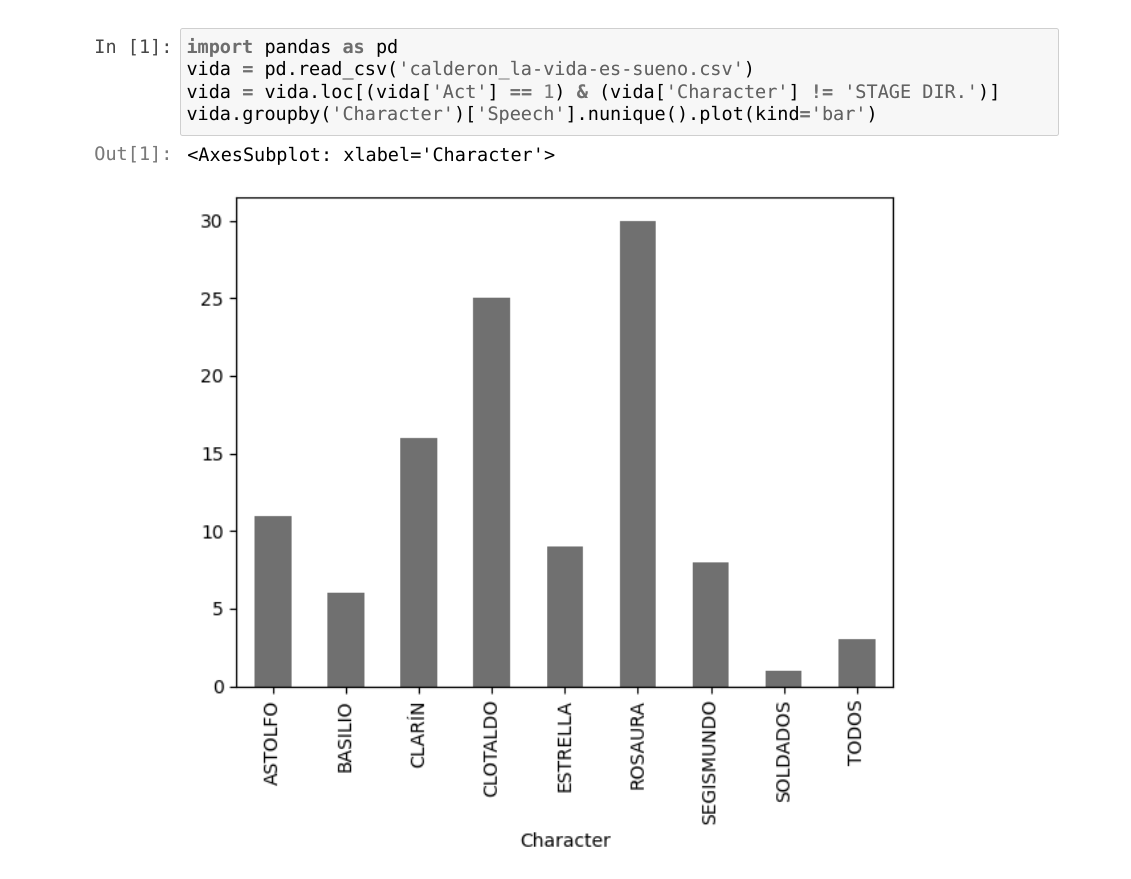
\includegraphics{images/pandasplot.png}}                             
	\caption{Ejemplo de aplicación.}
	\label{fig:pandasplot}
\end{figure}


La tabla permite un uso flexible y obtener información de manera rápida y sencilla. Por ejemplo, pueden compararse cuántas líneas dice cada personaje o, ya que disponemos del texto en sí, contar palabras por personaje (\Cref{fig:pandasplot}); podría asimismo diferenciarse entre personajes\index{personaje} femeninos o masculinos, o seguir el grado de participación de cada uno a lo largo de las escenas en función de sus parlamentos\index{parlamento}. Conociendo esto de cada una de las obras de un corpus, podrían compararse entre sí, en masa incluso, para encontrar piezas que se salgan de la norma. Si se agrupan, podría observarse las diferencias entre épocas, autores, géneros, o en función de varias variables, como la evolución de un autor en la producción de un género concreto a lo largo del tiempo.
